\section{Approach Overview}
\label{sec:overview}

The goal is to infer for all memory objects of each target loop high-level
properties that enable parallelization with minimal bookkeeping and access
checks.
% maybe the under which option is needed here?
%
These properties are used to group memory objects into families of objects.
%Memory objects with the same properties are grouped into the same family of
%objects.
The runtime system leverages each family's properties to maximize performance.
%
Even though, categorization of memory objects has been explored in prior
work~\cite{johnson:12:pldi, kim:12:cgo, corD},
%
the selection of properties and the assumptions under which these properties are
inferred drastically changes the parallelization profitability.  This section
explains how this work addresses these two problems more effectively than prior
work.
%to reduce speculative parallelization overheads compared to prior work.


%\subsection{Memory Object Properties}
\subsection{What Memory Object Properties?}

DOALL parallelization is \textit{applicable} when the loop's memory objects
belong to one of these categories: (i) private~\cite{privateer,LRPD} (does not
partake in any loop-carried memory flow); (ii) read-only~\cite{tian:10:pldi,
johnson:12:pldi}; (iii) local~\cite{tian:10:pldi, johnson:12:pldi,clusterDoall}
(allocated and de-allocated within the same iteration); and (iv)
reduction~\cite{privateer,LRPD_the_one_withreductionPriv} (participate in a
reduction operation only).
%

Ensuring correct live-out memory state often requires extensive bookkeeping,
during parallel execution, for the write footprint of private objects. To make
parallelization more \textit{profitable}, this work expresses more properties
for private memory objects. Private objects could additionally (a) be
independent~\cite{ARRAY_privatization} (no loop-carried false dependences); (b)
have loop-invariant condition for last update within the
loop~\cite{ARRAY_privatization}; (c) have predictable live-out content;
%(not found in prior work);
or (d) have only local accesses (allocated outside the loop, but all
accesses are contained within the loop execution).
%
%Private properties (a), (b) have been explored before in the context of static
%parallelization~\cite{ARRAY_privatization}, but never before in speculative
%parallelization systems (maybe in LRPD). No prior work leveraged property (c).
%
Table~\ref{tab:priv_types} summarizes how these properties can facilitate more
efficient parallelization compared to just inferring that a memory object is
private. In short, inference of any of these four private properties allows
complete elimination of bookkeeping and access checks. Prior software
speculative systems with extended support of privatization (Privateer~\cite{},
ClusterDoall~\cite{}) are only able to infer the simple private property and
thus always require costly checks or monitoring.

\centering
\tiny
\begin{tabular}{|c|c|c|c|c|c|c|c|c|}
  \hline
  Type of Private &
  Overlap         &
  Spec Privatization &
  Other Spec Allowed    &
  Loads Checks  &
  Store Checks    &
  Last-Write Detection &
  CoW Mapping &
  Copy-out to Main \\

%%%%%%%%%%%%%%%%%%% Shared %%%%%%%%%%%%%%%%%%%%%%%%%%
 \hline
 Shared & No & - & - & - & - & - & - & - \\
 \hline
%%%%%%%%%%%%%%%%%%% Local %%%%%%%%%%%%%%%%%%%%%%%%%%
 Local Private & Any & - & $\checkmark$ & - & - & - & $\checkmark$ & - \\
 \hline
%%%%%%%%%%%%%%%%%%% Overwrite %%%%%%%%%%%%%%%%%%%%%%%%%%
 Kill Private & Complete & - & $\checkmark$ & - & - & - & $\checkmark$ &
$\checkmark$ \\
 \hline
%%%%%%%%%%%%%%%%%%% Conservative Private %%%%%%%%%%%%%%%%%%%%%%%%%%
 Static Private & No/Partial & - & $\checkmark$ & - & - &
 $\checkmark$ & $\checkmark$ & $\checkmark$ \\
 \hline
%%%%%%%%%%%%%%%%%%% Specpriv Private %%%%%%%%%%%%%%%%%%%%%%%%%%
 Privateer Private & Any & $\checkmark$ & $\checkmark$ & $\checkmark$ & $\checkmark$ &
 $\checkmark$ & $\checkmark$ & $\checkmark$ \\
 \hline
\end{tabular}




%\subsection{How to Classify?}
%\subsection{How to Infer Memory Object Properties \\ Without Expensive Runtime
%Costs?}
\subsection{How to Infer Memory Object Properties?}

%Classifying memory objects
Characterizing the behavior of memory objects requires
%(i) identification of accesses to this object within the loop and
(i) mapping memory accesses to objects and (ii) analysis of the dependences that
these accesses introduce.
% characterize accesses
This work attempts to satisfy these two requirements by using a combination of
cheap-to-validate speculative assumptions and static analysis. For almost all
the memory objects of the evaluated benchmarks, this combination was sufficient
and no use of memory speculation or expensive bookkeeping was required.

%\paragraph{Determine accesses of memory objects:}
\paragraph{Map accesses to underlying memory objects:}
%
Static analysis can handle this problem for several cases of statically
allocated objects.
%
However, this task often becomes too challenging for static analysis for
general-purpose programs with unrestricted pointers, dynamic allocation, and
type casts.
%
%Briefly, this task entails ...  Challenges include points-to mapping from
%pointers to memory objects, different objects created by the same static
%instruction, unrestricted pointers presence of ``disguised''
%pointers~\cite{citation3_from_privateer}.  (not all pointer values are
%necessarily visible in the IR).
%
%These challenges often necessitate use of speculation.
Thus, in some cases use of speculation is necessary.
%
A points-to profiler can identify this mapping of memory accesses to underlying
memory objects.
%
Validating this points-to profiling information at the memory object granularity
would be expensive.
%instead of checking at runtime that each individual memory access points to the
%correct set of underlying objects,
%
%To enable cheap validation, it groups together memory objects with the same
%access pattern to a few heaps and only validates at runtime the correctness of
%points-to heap mapping.
%
% To reduce sensitivity to memory layout, Privateer speculativelyseparates
% memory objects
%
Same as in Privateer~\cite{johnson:pldi:12}, since all memory objects of the
same family share the same properties, inexpensive points-to family validation
is sufficient.
%
%TODO: maybe add one extra sentence here to explain why it is called separation
%spec or explain it more
%Inexpensive checks with neither bookkeeping nor inter-worker communication
%ensure that all accesses point to the correct heap.
%
%For example, the read-only family contains objects that speculatively map to
%read-only memory operations.  namely all the memory access have the read-only
%property.
%
This speculative scheme is called separation speculation.
%
%In contrast with Privateer~\cite{johnson:pldi:12}, we decouple separation
%speculation from characterizing memory accesses.
Note that Privateer's monolithic design of classification entangles separation
speculation with memory speculation and other profiling-based information
resulting in high runtime overhead (see section~\ref{eval}).
%
In contrast with Privateer, this work employs a modular design where separation
speculation is decoupled and can be used in conjunction with any other
cheap-to-validate speculation or static analysis to infer memory object
properties. This modularity leads to better planning and selection of minimum
cost solutions.

\paragraph{Dependence Analysis:}

%
Traditionally, dependence analysis (static, dynamic or speculative) in
speculative parallelization only attempts to completely remove dependences.
%
If a dependence cannot be removed even with usage of speculation, because
it is a real dependence that frequently manifests at runtime, no useful
information is provided related to this dependence.
%
Static analysis though, even if it failed to disprove a dependence, could
still infer some useful property for this dependence or the dependent
instructions.
TODO: briefly mention cases of annotations or nothing
Mention static analysis and speculative techniques used to annotate edges
or vertices

%Combining static with cheap-to-validate speculative analysis also
%enables property inference for efficient privatization.
%%
%Prior parallelization systems
%%~\cite{smtlite:09:pldi, kim:12:cgo, johnson:17:cgo}
%use static analysis or speculation mainly to remove memory
%dependences.  Sometimes though some dependences are real and cannot be
%removed via any kind of analysis.
%%For example,
%In particular, reuse of data structures creates cross-iteration false
%(output and anti) memory dependences.
%%
%In this scenario, analysis passes and speculative information can
%still express some useful properties for these dependences or the
%dependent instructions.  This partial information can be combined to
%infer a higher level property that enables more efficient
%parallelization.
%
%% isn't that what transformation do anyway? query analysis for
%% properties?  but we present a structured way to express that?  how
%% do analysis know what's useful.


%gives info to transforamtion.
%maybe in conjuction with other info from other analysis can enable a
%transformation efficiently
%some information that could enable a transformation enable more
%efficient parallelization

Explain inference of properties. Move that to next section.

One such property
that is explored in this paper is related to output dependences.  We refer
to this property as \textit{overwrite} and it expresses that the
destination operation of the dependence overwrites, in every iteration of
the target loop, the write footprint of the source operation.
%
%This information in conjunction with other static or speculative
%information infers that a private object has the property of
%loop-invariant condition for last update.
If all dependences related to a private object have the \textit{overwrite}
property then the private object has loop-invariant condition for last
update. In this case the last executed iteration has the correct live-out
memory state for this object and thus there is no need to monitor writes
for this memory object.

Maybe some of this info should be mention in the next section.
HERE briefly mention all the options.
Mention overwrite in the example subsection maybe


Value prediction can detect memory locations with loop-invariant values.
Not just remove dependences, add the annotation and remove cost of
monitoring wrties.
Loaded value re-interpreted as a store and kills all other RAW.

Independent can be infered by just disproving all output dependences. This
proves that there is no overlapping of writes.


Regarding dependence removal, prior work only used static analysis and
speculative assumptions in a sequence, operating independently of each
other.
%
This work suggests that exposing cheap-to-validate speculative assumptions
to static analysis can enable removal of memory dependences that would
otherwise require memory speculation.
TODO: add examples here
Figure out when to mention details about forms of collab. Probably in the
next section. Here just mention the techniques involved

For more details refer to section~\ref{collab}.


%Prior work only attempted to use static analysis and speculative assumptions
%separately to remove different dependences. If static analysis or speculative
%assumptions are unable to remove a dependence on their own, then there no
%collaboration between static analysis nor partial info to be used by
%transformations.


%In the past, privateer monolithically combined separation logic with
%mem spec to infer properties.
%no usage of static analusos/

%Mention the two speculative ones
%plus the usage of separation logic
%and the rest are the analysis algorithms from CAF


%First, a quick description of the used static and speculative analyses in our
%example:
%%
%\begin{itemize}
%%
%\item \textit{Static Analysis} (see ~\cite{johnson:17:cgo} for more information)
%%
%  \begin{itemize}
%%
%  \item \textit{Alias Analysis}: an ensemble of analysis algorithms that
%determine whether the footprint of an operation alias the footprint of another
%operation.
%%
%  \item \textit{Kill-Flow}: searches for killing operations along all feasible
%paths between two operations. It searches blocks which post-dominate the source
%of the queried dependence and dominate the destination.
%%
%  \item \textit{No-Capture Source}: identifies global variables or allocators
%whose address is never captured. Such objects can only be referenced through
%addresses computed from the object's name. The algorithm, thus, can enumerate,
%transitively, all uses of that object.
%%
%\end{itemize}
%%
%\item \textit{Speculative Analysis}
%%
%\begin{itemize}
%%
%  %\item \textit{Loop-Invariant Loaded Value Prediction}:
%  \item \textit{Value Prediction Speculation~\cite{}}: identifies, using
%value-prediction, profiling the predictable outcome of certain instructions.
%%cite F.  Gabbay  and  A.  Mendelson.    Can  program  profiling  supportvalue
%%prediction?
%%
%  \item \textit{Control Speculation~\cite{}}: identifies, using edge profiling,
%speculatively dead code and asserts absence of memory dependences to or from
%speculatively dead operations.
%%cite W. Y. Chen, S. A. Mahlke, and W. W. Hwu.  Tolerating first levelmemory
%%access latency in high-performance systems
%%
%\end{itemize}
%%
%\end{itemize}
%%

%Private detection requires privatization criteria and actual detection.

%conditional update makes it hard to find last store
%  but in some cases ctrl spec can be used to remove this problem!
%and remove RAW and allow cheap privitization


\lstset{basicstyle=\ttfamily, numbers=left, numberstyle=\tiny,
  stepnumber=1, numbersep=5pt}

\begin{figure*}
\centering
\subfloat[Privateer~\cite{johnson:12:pdli}]{
  \centering
  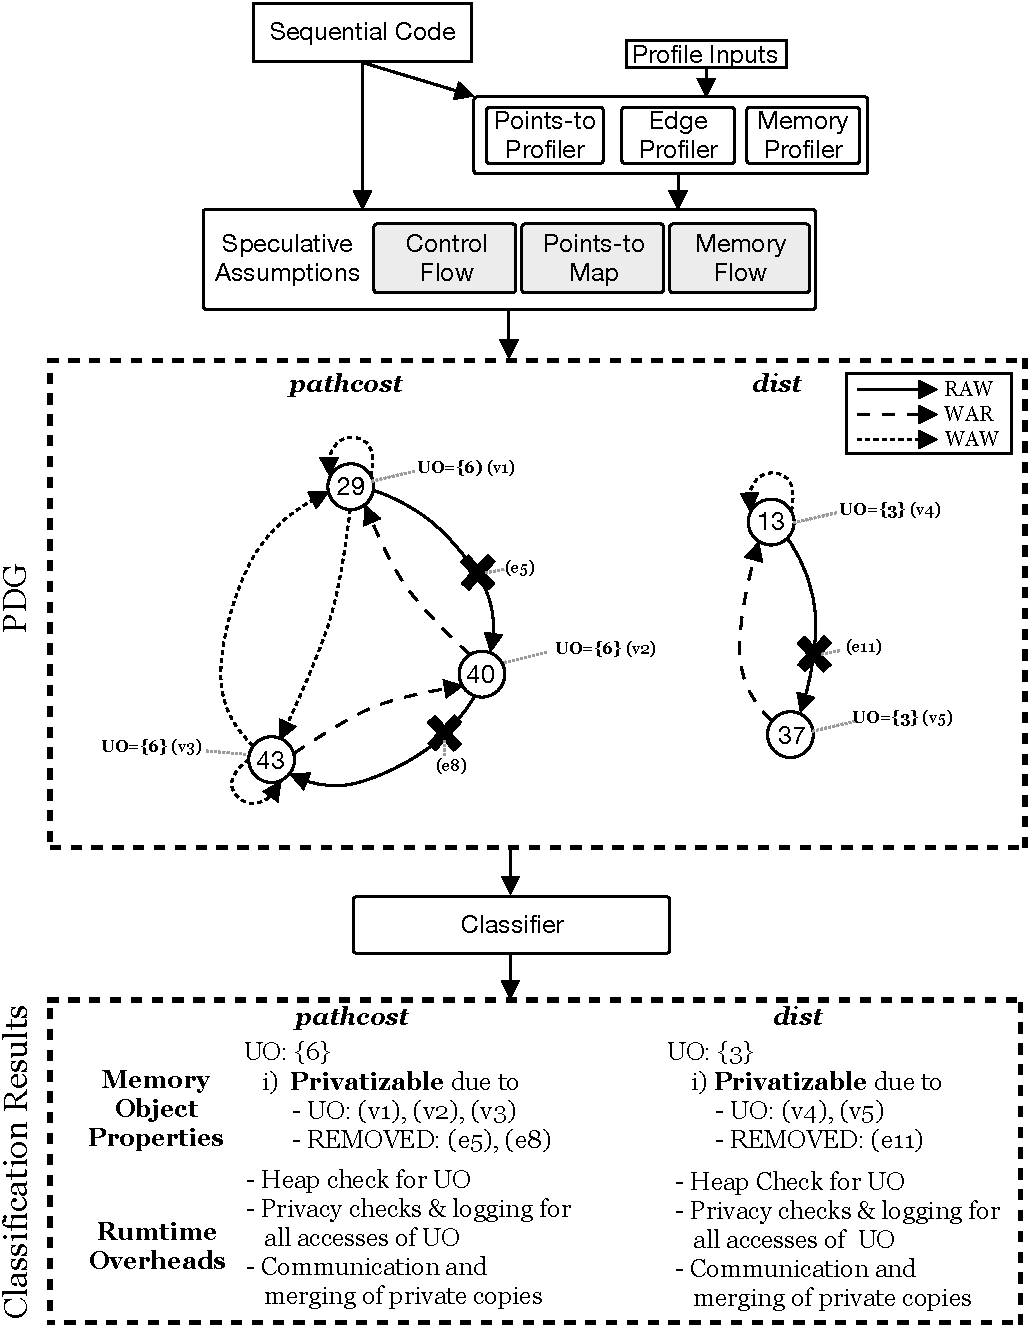
\includegraphics[width=0.46\textwidth]{figures/privateer-example-crop}
}
\qquad
\subfloat[This work]{
  \centering
  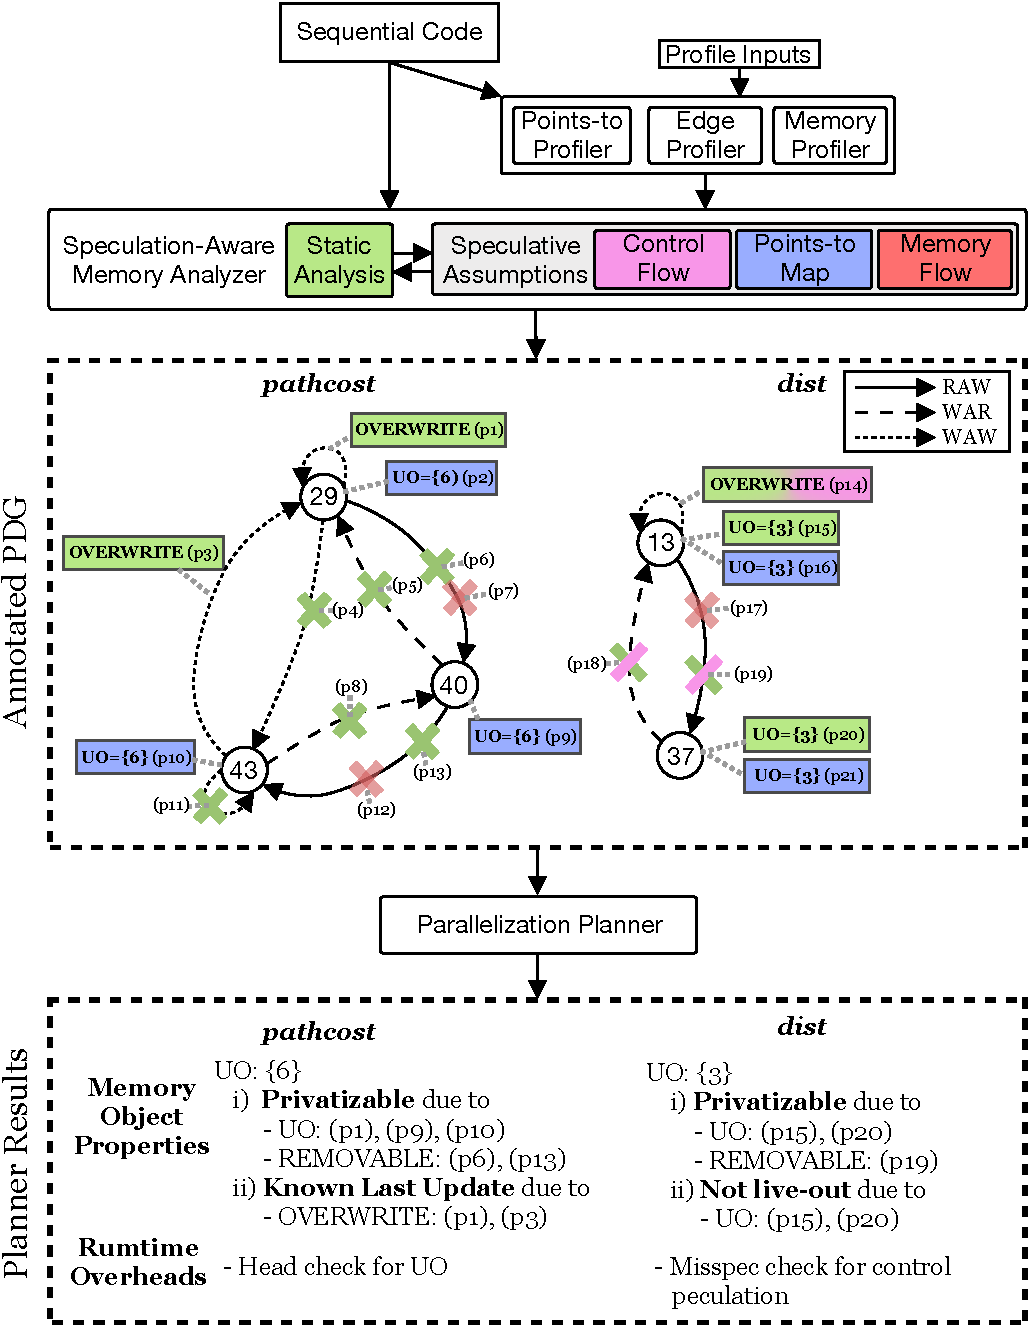
\includegraphics[width=0.46\textwidth]{figures/perspective-example-crop}
}
\caption{Property inference comparison of Privateer with LSD for memory
objects \textit{pathcost} and \textit{dist} of the hot loop of \textit{dijkstra}}
\label{fig:dijkstra_motivation_comparison}
\end{figure*}

\begin{figure*}
\centering
\scriptsize
\subfloat[Privateer~\cite{johnson:12:pdli}]{
  \centering
  \begin{minipage}{8.55cm}
  \begin{lstlisting}[morekeywords={pathcost}, belowskip=0pt, firstnumber=1,
name=dij_checks]
int *pathcost; // dyn alloc 1-D N
int *adj; // dyn alloc 2-D NxN
int dist, v, src, i;

for (src=0; src<N; src++) {
\end{lstlisting}

\begin{lstlisting}[morekeywords={pathcost}, aboveskip=0pt,belowskip=0pt,backgroundcolor=\color{lightgray},
firstnumber=auto, name=dij_checks]
  // Privacy Check
  private_write(pathcost, N*sizeof(int));
\end{lstlisting}

\begin{lstlisting}[morekeywords={pathcost},aboveskip=0pt, belowskip=0pt, firstnumber=auto,name=dij_checks]
  for (i=0; i<N; i++)
    pathcost[i] = inf;

  enqueue(src, 0);
  while (!emptyQ()) {
    dequeue(&v, &dist);
    for (i=0; i<N; i++) {
      nDist = adj[v][i] + dist;
\end{lstlisting}

\begin{lstlisting}[morekeywords={pathcost}, aboveskip=0pt,belowskip=0pt,backgroundcolor=\color{lightgray},
firstnumber=auto, name=dij_checks]
      // Privacy Check
      private_read(pathcost, sizeof(int));
\end{lstlisting}


\begin{lstlisting}[morekeywords={pathcost}, aboveskip=0pt, belowskip=0pt, firstnumber=auto,name=dij_checks]
      if (pathcost[i] > nDist) {
\end{lstlisting}

\begin{lstlisting}[morekeywords={pathcost}, aboveskip=0pt,belowskip=0pt,backgroundcolor=\color{lightgray},
firstnumber=auto, name=dij_checks]
        // Privacy Check
        private_write(pathcost, sizeof(int));
\end{lstlisting}

\begin{lstlisting}[morekeywords={pathcost}, aboveskip=0pt, belowskip=0pt, firstnumber=auto,name=dij_checks]
        pathcost[i] = nDist;
        enqueue(i, nDist);
      }
    }
  }
}
\end{lstlisting}

  \end{minipage}
}
\qquad
\qquad
\subfloat[This work]{
  \centering
  \begin{minipage}{7.2cm}
  %\begin{lstlisting}[morekeywords={pathcost}, belowskip=0pt, firstnumber=1,
%name=dij_checks]
%int *pathcost; // dyn alloc 1-D N
%int *adj; // dyn alloc 2-D NxN
%int dist, v, src, i;


\begin{lstlisting}[morekeywords={pathcost,dist}, belowskip=0pt,
firstnumber=10, name=dij_checks, showlines=true]
int dequeue() {
  if (!emptyQ()) {


\end{lstlisting}

\begin{lstlisting}[morekeywords={pathcost,dist}, aboveskip=0pt, belowskip=0pt,
firstnumber=13, name=dij_checks]
    dist = ...
    ...
  }
\end{lstlisting}

  \begin{lstlisting}[morekeywords={pathcost}, aboveskip=0pt,belowskip=0pt,backgroundcolor=\color{lightgray}, firstnumber=auto, name=dij_checks]
  else // 0% added overhead
    misspec("Control misspec in dequeue()");
\end{lstlisting}

\begin{lstlisting}[morekeywords={pathcost,dist}, aboveskip=0pt, belowskip=0pt,
firstnumber=auto, name=dij_checks,showlines=true]
}

void worker_loop(int start, int N, int step) {

\end{lstlisting}

  \begin{lstlisting}[morekeywords={pathcost}, aboveskip=0pt,belowskip=0pt,backgroundcolor=\color{lightgray},
  firstnumber=auto, name=dij_checks,showlines=true]
  // Separation Local Check -- < 0.001% added overhead
  check_heap(pathcost, OVERWRITE_PRIVATE);
  \end{lstlisting}

\begin{lstlisting}[morekeywords={pathcost}, aboveskip=0pt,
belowskip=0pt, firstnumber=24,name=dij_checks,showlines=true]

  for (src=start; src<N; src+=step) {


\end{lstlisting}
\begin{lstlisting}[morekeywords={pathcost,dist}, aboveskip=0pt,
belowskip=0pt, firstnumber=28,name=dij_checks,showlines=true]
    for (i=0; i<N; i++)
      pathcost[i] = inf;

    enqueue(src, 0);
    while (!emptyQ()) {
      int v = dequeue();
      for (i=0; i<N; i++) {
\end{lstlisting}
\begin{lstlisting}[morekeywords={pathcost,dist,nDist}, aboveskip=0pt,
belowskip=0pt, firstnumber=auto,name=dij_checks,showlines=true]



        nDist = adj[v][i] + dist;
\end{lstlisting}
\begin{lstlisting}[morekeywords={pathcost}, aboveskip=0pt,
belowskip=0pt, firstnumber=auto,name=dij_checks,showlines=true]


        if (pathcost[i] > nDist) {


\end{lstlisting}
\begin{lstlisting}[morekeywords={pathcost}, aboveskip=0pt,
belowskip=0pt, firstnumber=auto,name=dij_checks]
          pathcost[i] = nDist;
          enqueue(i, nDist);
        }
      }
    }
\end{lstlisting}

\begin{lstlisting}[morekeywords={pathcost,dist}, aboveskip=0pt,
belowskip=0pt, firstnumber=auto,name=dij_checks,showlines=true]
  }
\end{lstlisting}

\begin{lstlisting}[morekeywords={pathcost},
aboveskip=0pt,belowskip=0pt,backgroundcolor=\color{lightgray},
firstnumber=auto, name=dij_checks,showlines=true]
  // only last iter's pathcost array
  // needs to be communicated -- < 1% added overhead
  if (src == N-1+step)
    communicate_pathcost();
\end{lstlisting}

\begin{lstlisting}[morekeywords={pathcost}, aboveskip=0pt,
belowskip=0pt, firstnumber=auto,name=dij_checks]
}
\end{lstlisting}

  \end{minipage}
}
\caption{Source code comparison of Privateer with LSD for parallelized hot loop
of \textit{dijkstra}. Checkpointing occurs every several (long running) loop iterations, thus its
overhead is negligeable for \textit{dijkstra}. Logging and checks
during loop execution dominate the overheads.}
\label{fig:dijkstra_motivation_comparison_source_code}
\end{figure*}



\paragraph{Example:}
This example underlines inefficiencies and limitations of prior work and
showcases how the combination of static analysis with cheap-to-validate
speculative assumptions can infer program properties that enable scalable
parallelization.
%
Consider the code in
Figure~\ref{fig:dijkstra_motivation} (taken from MiBench~\cite{} benchmark
dijkstra, used in the evaluation of Privateer~\cite{}).
%
Reuse across iterations of the \textbf{pathcost} array and global variable
\textbf{dist} creates cross-iteration false dependences that inhibit
parallelization.
%
Privatization enables parallelization of this loop by creating private
copies of \textbf{pathcost} and \textbf{dist} memory objects for every
worker.
%
From prior work, Privateer~\cite{johnson:12:pldi} is the only automatic
system to support privatization of dynamically allocated objects, like
\textbf{pathcost}, even in the presence of unrestricted pointers.
%
Figure~\ref{fig:dijkstra_motivation_comparison} compares the property
inference property of Privateer compared to this work.
The difference is that

Figure~\ref{fig:dijkstra_motivation_comparison_source_code} compares the
resulting parallelized versions (in a simplified form) for Privateer and
this work. The code includes all the added checks, logging and handling
live-out overheads. The code changes are marked with the average added
overhead over the useful work of each worker.
It is clear that Privateer introduces a lot of added overhead considerably
limiting its profitability. XXX on the other side ..


Privateer would choose to just do simple privatization with mem spec.
The spec-aware analyzer allows removal of mem spec and efficient
privatization in this case.

\begin{itemize}
\item
Privatization of these memory objects requires:
\begin{enumerate}
\item
identification of all accesses of these objects
    within the loop
\item
absence of cross-iteration flow
     dependences on each of these accesses
\end{enumerate}

\end{itemize}


Remove text from figure 1. Just add some here, the rest has been explained
earlier.
Real dependnecs prevent
DOALL can become applicable if these two objects are proven to have the
private property.

We compare our approach where we combine static analysis with cheap-to-validate
with privateer's monolithic approach that over-speculates and is limited by high
runtime overheads.

We initially present the compilation flow for both approaches, then the
resulting parallelized code and finally the flow of live-in and live-out memory
data.

Whilst the private property is enough for DOALL
Notice that we infer an additional property that improves the profitability
of parallelization.

%Note that anti-dependences are ignored since both systems use
%process-based runtime systems.

For inferring the property that a memory object has the locally-accessed
property, it suffices to identify all accesses of the memory object. If all
these accesses are within the loop then the memory object has the
locally-accessed property.


%dijkstra (used in the evaluation of Privateer~\cite{}) to showcase how static
%analysis along with cheap-to-validate speculative assumptions can infer
%high-level program properties and enable scalable parallelization.
%%
%We focus on two memory objects that would cause inefficiencies on prior
%parallelization systems.
%%
%For each of these objects, we examine how we can tackle DOALL parallelization
%inhibitors; in particular loop-carried memory dependences, and exhibit the
%multiplicative effect of collaboration in terms of analysis accuracy.
%


%%showcases how fine-grained collaboration between static analysis and speculative
%%assumptions can infer high-level program properties without the need for
%%expensive memory speculation.
%
%%Dependence has three conditions. We say there is a memorydependence  from
%%instructioni1to  instructioni2iff(alias)the footprint of operationi1may-aliasthe
%%footprint ofi2, and(feasible-path) there is a feasible path of execution
%%fromi1toi2which (no-kill) does not contain an operation which over-writes the
%%common memory footprint. Footprint denotes theset of memory locations read or
%%written by the instruction.
%
%1) global object \textit{g\_qCount}
%
%\textbf{Static analysis and inexpensive speculation in isolation}:
%%
%%Analysis Results:
%Static analysis cannot disprove all loop-carried RAW and WAW dependences on
%accesses of g\_qCount.
%%
%Profile information indicates that the first load of g\_qCount in each iteration
%always returns zero.  Using this information, value prediction removes the
%loop-carried RAW dependence sinking on this load.
%%
%Removal of this dependence prevents usage of memory speculation for this
%particular load.
%%
%Presence of WAW dependences though necessitates privatization of the memory
%object, and value prediction cannot reason about store instructions and cannot
%give any additional information related to output dependences.
%%
%%Cost
%The cost in this case includes the validation overhead for value prediction
%(perform load before loop exits or on backedges and compared predicted value
%with loaded value) and the privatizaition cost (monitor stores participating in
%the WAW dependences to determine last written value). Bookkeping for
%privatization is the dominant cost as it requires updating metadata multiple
%times per loop iteration (given that some stores are within inner loops).
%%dynamic resolution to determine last written value
%
%
%\textbf{Collaboration of static and speculative analysis}:
%%
%This value prediction can be seen as a store before the first load of g\_qCount
%that kills any data flow for this memory object from previous iterations.
%%
%An extended speculative analysis removes, similarly to the first case, the
%loop-carried RAW dependence, but additionally queries alias analysis for
%must-aliasing accesses with the load's address. If these accesses are dominated
%by the load, then loop-carried RAW or WAW dependences from or to these accesses
%can be ignored.
%%
%This remvoes the need to perform dynamic resolution of the last written value;
%the final content of this memory location is predictable.
%%any action to log (for last write) any of these individual memory operations.
%%
%%Interestingly, this case of privatization goes beyond the classical definition
%%of privatization definition~\cite{tu-padua-array-privatization-1994}  that
%%requires that every load of a privatizable element is preceded by a store to
%%the element in the same iteration of the loop. In this scenario, global
%%variable g\_qCount is first loaded at every iteration, a data flow exists.
%%
%%
%The cost in this case only includes the small validation overhead for value
%prediction. There is no bookkeping cost for privatization.
%%
%No prior work could detect and so effectively handle this new case of
%privatization.
%%- privatization cost: none avoid dynamic resolution to determine last written
%%value (live-out value)
%
%%TODO: use this first
%2) global object \textit{iPrev}
%
%- speculative assumption: the branch "if (qHead)" is always taken (control speculation)
%
%- static analysis: alias analysis, killflow, noCaptureGlobal analysis passes
%
%- validation cost: no validation cost for control spec (just misspecs if branch
%  is not taken)
%
%- Using the speculative assumption, killflow analysis can infer that the store
%  in line 15 kills all other accesses of this global
%variable (killed operations are identified by quering alias analysis). Given this
%property, any RAW loop-carried dependence is disproved.  Additionally, static
%analysis can enumerate all uses of this global, since it is not captured, and
%detect that this global is used only within this loop, namely it is not a
%live-out.  Thus, there is no need to log stores and keep track of the last
%written value to it.
%
%%3) TODO: example with blackscholes
%
%For all the above memory objects, Privateer~\cite{}, the state-of-the-art DOALL
%system that we mainly compare against, would require expensive logging on most
%of their accesses,
%%either for validation checks or for identifying who wrote last what
%yielding sub-optimal speedups as clearly exhibited by our experimental results
%in section ~\ref{eval}.
%%all these objects are classified as privatizable by Privateer
%
%Note that our framework is not limited to static global allocations.  It can
%handle linked or recursive data structures, pointers,type  casts,  and  dynamic
%allocation.
%
%%use alvinn for value pred + alias analysis
%
%%Note that WAR dependences can be ignored thanks to the process-based runtime
%%system.


%\lstset{basicstyle=\ttfamily, numbers=left, numberstyle=\tiny,
%  stepnumber=1, numbersep=5pt}
%\begin{figure*}[t]
%  \centering
%  \scriptsize
%  \subfloat[dijkstra -- predictable]
%  {
%    \label{fig:dijkstra}
%    \begin{minipage}{7.5cm}
%      \begin{lstlisting}[morekeywords={g_qCount},belowskip=0pt]
// predicted to be 0 at start of every iteration
int g_qCount = 0;

for ( int i = 0; int j = N/2; i < N; i++, j++ ) {
  ...
  enqueue( i, 0, NONE );
  g_qCount++;
  while ( g_qCount ) {
    dequeue( &iNode, &iDist, &iPrev );
    g_qCount--;
    for ( k = 0; k < NUM_NODES; k++ ) {
      ...
      if ( valid_node ) {
        ...
        enqueue( i, iDist + iCost, iNode );
        g_qCount++;
      }
    }
  }
  ...
}

\end{lstlisting}

%    \end{minipage}
%  }
%  \hspace{0.5cm}
%  \subfloat[dijkstra -- overwrite]
%  {
%    \label{fig:blackscholes}
%    \begin{minipage}{7.5cm}
%      \input{figures/dijkstra_overwrite_code}
%    \end{minipage}
%  }
%\end{figure*}
%
%
%
%
%\begin{figure*}[t]
%  \centering
%  \scriptsize
%  \subfloat[gemm -- shared]
%  {
%    \label{fig:gemm}
%    \begin{minipage}{7.5cm}
%      \begin{lstlisting}[escapeinside={~}{~}, belowskip=0pt]
for ( i = 0; i < ni; i++ ) {
  for ( j = 0; j < nj; j++ ) {
    C[i][j] *= beta; 
    for ( k = 0; k < nk; ++k )
      C[i][j] += alpha * A[i][k] * B[k][j];
  }
}
\end{lstlisting}

%    \end{minipage}
%  }
%  \hspace{0.5cm}
%  \subfloat[blackscholes -- overwrite]
%  {
%    \label{fig:blackscholes}
%    \begin{minipage}{7.5cm}
%      % look in Nick's motivation.tex for formatting
\begin{lstlisting}[morekeywords={prices}, belowskip=0pt]
for ( j = 0; j < NUM_RUNS; j++ ) {
  for ( i = 0; i < numOptions; i++ ) {
    prices[i] = BlkSchlsEqEuroNoDiv(
      sptprice[i], strike[i],
      rate[i], volatility[i], otime[i],
      otype[i], 0);
  }
}
\end{lstlisting}

%    \end{minipage}
%  }
%\end{figure*}
%\begin{figure*}[t]
%  \centering
%  \scriptsize
%  \subfloat[052.alvinn -- stack local]
%  {
%    \label{fig:alvinn_local}
%    \begin{minipage}{7.5cm}
%      \begin{lstlisting}[morekeywords={psum_array},belowskip=0pt]
float psum_array[NHU+1]; // stack

for (epoch = 0; epoch < NUM_EPOCHS; epoch++) {
  ...
  for ( i = 0; i < NHU+1; i++ )
    psum_array[i] = 0;
  for( i = 0; i < NOU; i++ ) {
    for ( j = 0; j < NHU+1; j++ ) {
      ...
      psum_array[j] += delta[i] * weights[i][j];
      ...
    }
  }
  for ( i = 0; i < NHU+1; i++ )
    delta[i] = hidden[i] * (1 - hidden[i]) * psum_array[i];
  ...
}
\end{lstlisting}

%    \end{minipage}
%  }
%  \hspace{0.5cm}
%  \subfloat[dijkstra -- global local]
%  {
%    \label{fig:dijkstra}
%    \begin{minipage}{7.5cm}
%      \begin{lstlisting}[morekeywords={k},belowskip=0pt]
int k;

for ( int i = 0; int j = N/2; i < N; i++, j++ ) {
  ...
  j = j%N;
  if ( i == j )
    continue;
  else {
    ...
    while ( g_qCount ) {
      ...
      for ( k = 0; k < NUM_NODES; k++ ) {
        ...
      }
    }
  }
  ...
}

\end{lstlisting}

%    \end{minipage}
%  }
%\end{figure*}

% \begin{figure*}[t]
%   \centering
%   \scriptsize
%   \subfloat[covariance -- nospec-private]
%   {
%     \label{fig:covariance}
%     \begin{minipage}{7.5cm}
%       \begin{lstlisting}[morekeywords={symmat}, belowskip=0pt]
for ( j1 = 0; j1 < m; j1++ ) {
  for ( j2 = j1; j2 < m; j2++ ) {
    symmat[j1][j2] = 0.0;
    for ( i = 0; i < n; i++ )
      symmat[j1][j2] += data[i][j1] * data[i][j2];
    symmat[j2][j1] = symmat[j1][j2];
  }
}
\end{lstlisting}

%     \end{minipage}
%   }
%   \hspace{0.5cm}
%   \subfloat[052.alvinn -- real private]
%   {
%     \label{fig:alvinn_specpriv}
%     \begin{minipage}{7.5cm}
%       \begin{lstlisting}[morekeywords={output_act}, belowskip=0pt]
float output_act[NOU];

for (epoch = 0; epoch < NUM_EPOCHS; epoch++) {
  ...
  receiver = &output_act[0];
  end_receiver = &output_act[NOU - 1];
  for ( ; receiver <= end_receiver; ) {
    *receiver = 0.0;
    sender = &hidden_act[0];
    end_sender= &hidden_act[NHU];
    for (; sender <= end_sender; )
      *receiver += (*sender++) * (*weight++);
    *receiver = SIGMOID(*receiver);
    *receiver++;
  }
  ...
  for (ou = 0; ou < NOU; ou++) {
  	delta[ou] = (teach[ou] - output_act[ou]) *
      output_act[ou] * (1.0 - output_act[ou]);
  	...
  }
  ...
}
\end{lstlisting}

%     \end{minipage}
%   }
% \end{figure*}
